%\newpage 
%\section{Methodology}¨
%\chapter{Methodology}
%\label{sec:methodology}

\chapter{Review of state of the art anomaly detectors}
%\section{Evaluation of RX, LRX and ACAD }
%\label{sec:MATLAB_methodology}
\label{chapter:review_anomaly_detectors}
To evaluate the performance of the ADs considered in this task, models of the algorithms described in section \ref{sec:anomaly_detectors_theory} were developed in MATLAB, and tested on both hyperspectral image data from the Cuprite site \cite{Cuprite_data} gathered by the AVIRIS imager and synthetic images created by the author. The creation of the synthetic images are described in Section \ref{sec:synthetic_images}.
\\

The MATLAB hyperspectral toolbox \cite{MATLAB_hyperspectral_toolbox} was used for image preprocessing, visualization and for having a good starting point for developing further functionality. The toolbox included an implementation of the RX algorithm. A fork of the toolbox was made, available at \cite{MATLAB_hyperspectral_toolbox_fork}, to be able to do MATLAB implementations of LRX, ALRX and ACAD in order to evaluate the performance of the ADs. The most important scripts and functions from the forked toolbox are also located in appendix \ref{appendice:MATLAB_hyperspectral}.

\section{Experiments on Synthetic images}
\label{sec:synthetic_images}
To make an objective analysis  of the considered ADs performance, synthetic hyperspectral images with known anomalies were created. The images contained anomalies of various sizes, to test the ADs ability to detect variably sized anomalies. A similar test is also done in \cite{global_and_local_rx}. Figure 7(a) in \cite{global_and_local_rx} shows that the RX algorithm was not able to detect anomalies in the third and four column (anomalous pixels made up of >50\% abundance of the anomaly signature). The LRX exhibit slightly better anomaly detection accuracy in this test.
\\

The purpose of the synthetic images used in this thesis was to get objective metrics of the performance of the evaluated ADs. Two different metrics are important in order to evaluate the performance of the ADs; $false\_anomalies$ and $correctly\_predicted\_anomalies$. These metrics are defined in equation \ref{eq:false_anomalies_metric} and \ref{eq:correctly_predicted_anomalies_metric};
\begin{equation}
    false\_anomalies = predicted\_anomalies - true\_anomalies
    \label{eq:false_anomalies_metric}
\end{equation}

\begin{equation}
    correctly\_predicted\_anomalies= \frac{predicted\_anomalies\_in\_reference\_map}{reference\_anomalies}
    \label{eq:correctly_predicted_anomalies_metric}
\end{equation}

$predicted\_anomalies\_in\_reference\_map$ is the number of predicted anomalies that are correctly predicted anomalies. $reference\_anomalies$ are the number of true anomalies in the anomaly map. These metrics are important as they provide an objective way to evaluate the performance of the ADs, something that can not be done with real hyperspectral image data, unless one possesses a reference anomaly map to the real image data, which the author has not been able to find.  

% If this is bigger than >0, else 0

%\begin{equation}%    correctly\_predicted\_anomalies= \frac{true\_anomalies}{predicted\_anomalies}%    \label{eq:correctly_predicted_anomalies_metric}%\end{equation}

Synthetic images with different sizes and anomaly sizes were created to evaluate the performance of the ADs. Tests were done to get an objective evaluation of the considered ADs. To be able to compare to the tests done on images with a size of 200x200 as described in chapter 5.5.1 in \cite{hsueh_master_thesis} by Hsueh, these tests were mimicked. The synthetic image for this test can be seen in Figure \ref{fig:hsueh_image}. In addition, synthetic images with size of 30 x 30 pixels were created with an anomalous panel of size 2x2 inserted into the center of the images. This image scene is labelled $Sim30\_30AVIRIS$. The anomalous pixels are pure pixels with a spectral signature of Buddingtonite. These images has a background consisting of $33\%$ Alunite, $33\%$ Kalonite and $33\%$ Pyrope. Such a generated synthetic image can be seen in Figure \ref{fig:synthetic_30_30}. This figure displays spectral band 160.


%\begin{figure}[H]
%\begin{minipage}[]{.5\linewidth}
%\centering
%\subfloat[ 200 x 200 synthetic image.]{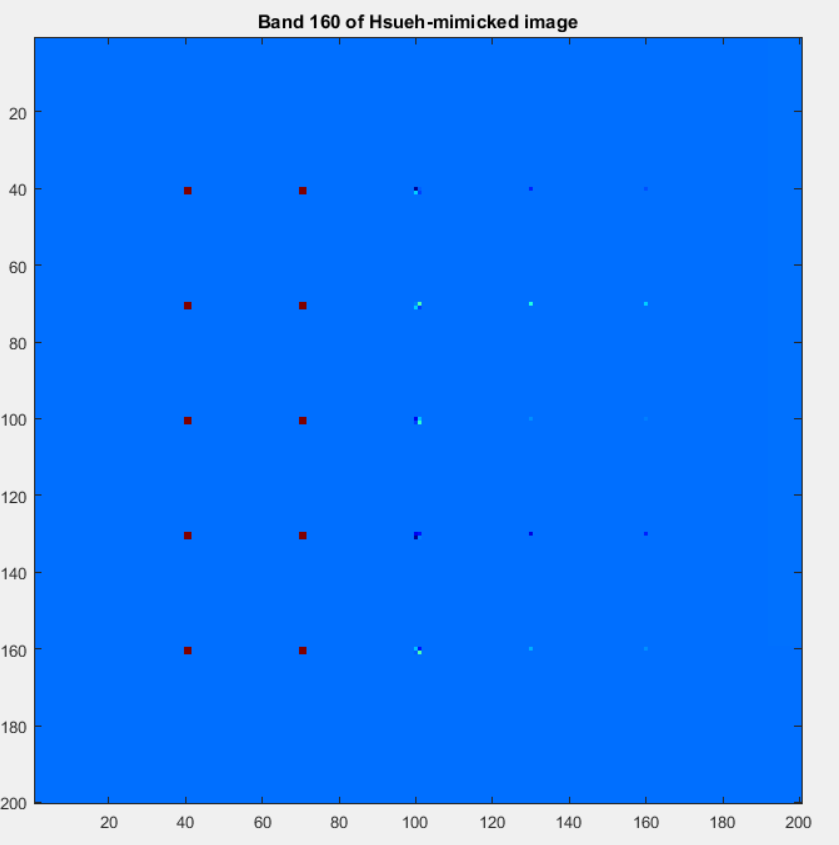
\includegraphics[scale=.25]{images/AD_testing/synthetic_images/band_160_hsueh_picture_without_gaussian_noise.PNG}}
%  %\caption{Lena 256 x 256 uncompressed. Used for testing of MATLAB SPIHT script.}
%  %\label{fig:lena_unc}
%\end{minipage}%
%\begin{minipage}[]{.5\linewidth}
%%\hspace*{-4m}
%\centering
%  \subfloat[Synthetic image with added Gaussian white noise with a SNR of 20:1.]{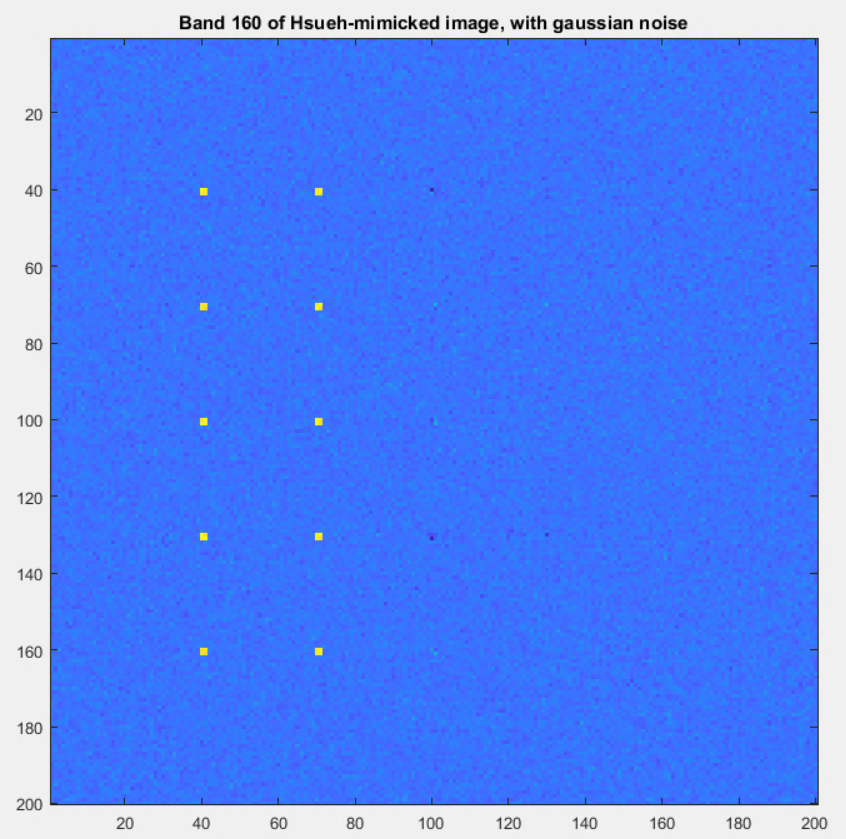
\includegraphics[scale=.25]{images/AD_testing/synthetic_images/band_160_hsueh_picture_with_gaussian_noise.PNG}}
%  %\caption{Lena 256 x 256 reconstructed after being compressed having 0.1 bpp, using the MATLAB SPIHT script. See appendix. }
%  %\label{fig:lena_comp}
%\end{minipage}


%\caption{First class of synthetic images: 200 x 200 synthetic image with 25 inserted anomaly panels as describe by Hsueh in \cite{hsueh_master_thesis}. Displaying spectral band 160. }
%\label{fig:hsueh_image}
%\end{figure}

\begin{figure}[H]
\centering
   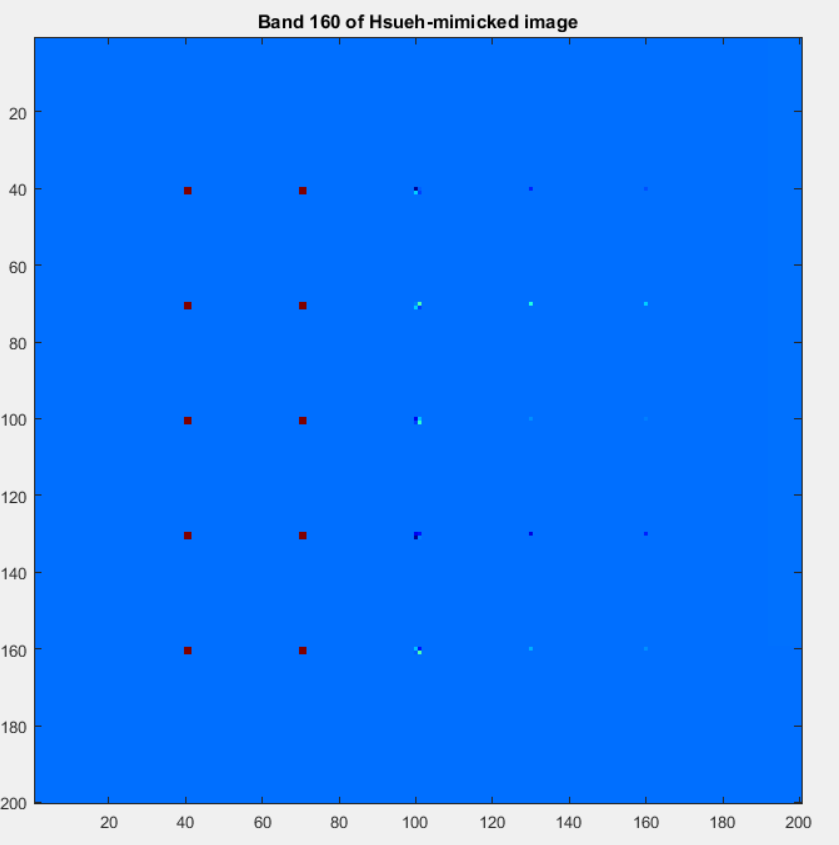
\includegraphics[scale=0.7]{images/AD_testing/synthetic_images/band_160_hsueh_picture_without_gaussian_noise.PNG}
  \caption{First class of synthetic images: 200 x 200 synthetic image with 25 inserted anomaly panels as describe by Hsueh in \cite{hsueh_master_thesis}. } 
  \label{fig:hsueh_image}
\end{figure}

\begin{figure}[H]
\centering
   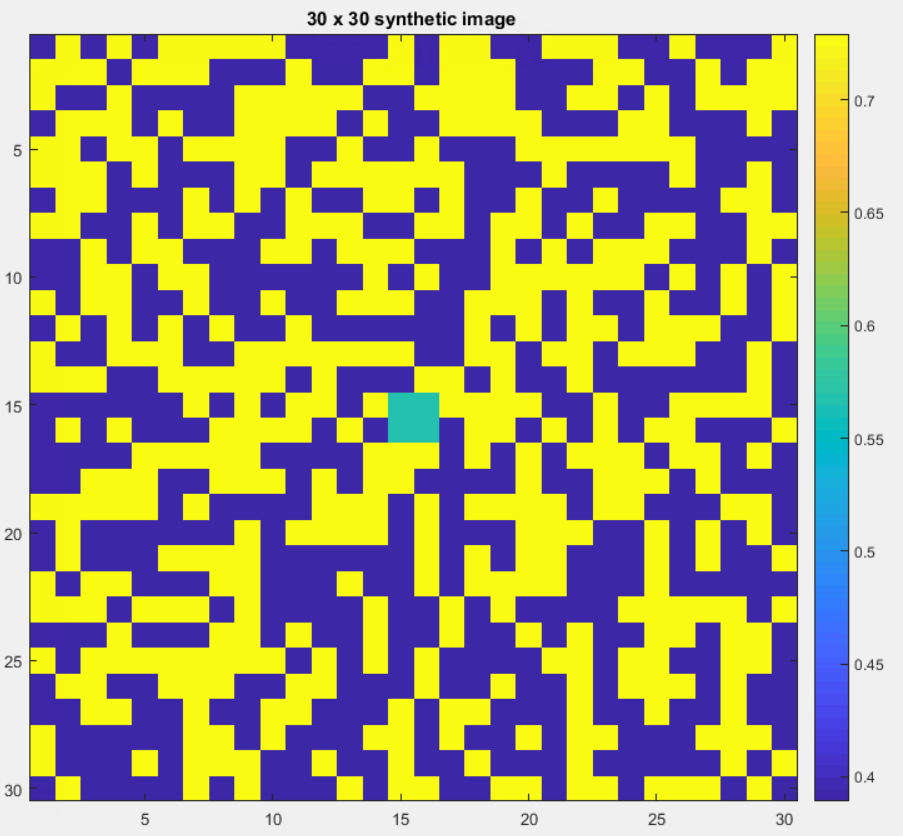
\includegraphics[scale=0.4]{images/AD_testing/synthetic_images/30_30_anomaly_image.PNG}
  \caption{Second class of synthetic images: Synthetic 30x30 image with an inserted 2x2 anomalous panel inserted into the center.} 
  \label{fig:synthetic_30_30}
\end{figure}


\\
A third class of synthetic images with a size of $100$ x $614$ pixels was also created, labelled $SimAviris01$. These images has a background consisting of $33\%$ Alunite, $33\%$ Kalonite and $33\%$ Pyrope. The anamalous pixels are pure pixels with a spectral signature of Buddingtonite, extracted from the Cuprite image scene \cite{ground_truth_cuprite}. Six different sized anomalous-target kernels were made, with a size of $1x1$, $2x2$, $5x5$, $10x10$, $15x15$, $20x20$ and $25x25$ pixels. Table \ref{tab:synthetic_images} describes the properties of $SimAviris01$.




\begin{table}[H]
\centering
\caption{Properties of $SimAviris01$ .Row and column locations are location of the center pixel in the kernel of size $K$ $\times$ $K$.}
\label{tab:synthetic_images}
\begin{tabular}{l|l|l|l}
\textbf{Scene} & \textbf{Row} & \textbf{Column} & \textbf{Anomaly size {[}pixels x pixels{]}} \\
SimAviris01    & 35           & 50              & 1x1                                         \\
SimAviris01    & 70           & 50              & 1x1                                         \\
SimAviris01    & 35           & 100             & 2x2                                         \\
SimAviris01    & 70           & 100             & 2x2                                         \\
SimAviris01    & 35           & 150             & 5x5                                         \\
SimAviris01    & 70           & 150             & 5x5                                         \\
SimAviris01    & 35           & 250             & 10x10                                       \\
SimAviris01    & 70           & 250             & 10x10                                       \\
SimAviris01   & 35           & 350             & 15x15                                       \\
SimAviris01    & 70           & 350             & 15x15                                       \\
SimAviris01    & 35           & 450             & 20x20                                       \\
SimAviris01    & 70           & 450             & 20x20                                       \\
SimAviris01    & 35           & 550             & 25x25                                       \\
SimAviris01    & 70           & 550             & 25x25                                      
\end{tabular}
\end{table}



\begin{figure}[H]
\hbox{\hspace*{-0}                                              
   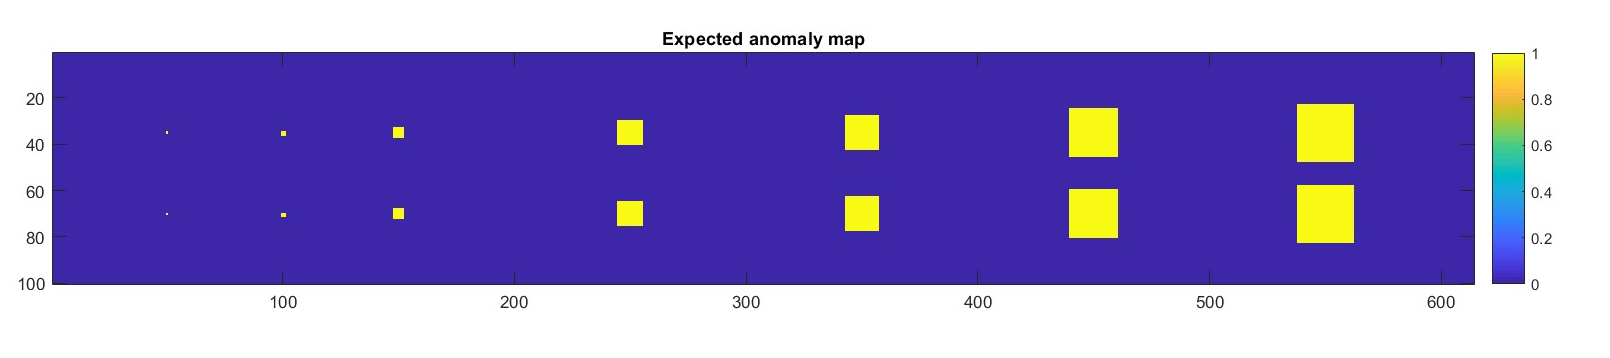
\includegraphics[scale=0.4]{images/AD_testing/synthetic_images/expected_anomaly_map.png}}
  \caption{Expected anomaly map for the third class of synthetic images created.} 
  \label{fig:anomaly_map_615_100}
\end{figure}


Since the RX and LRX AD does not build an anomaly map, the author defines anomalous pixels as pixels having a score of $\geqslant$ 75\% of the max value outputted from the RX AD or the LRX AD. This is done in order to be able to set the objective metrics $false\_anomalies$ and $correctly\_predicted\_anomalies$.

\subsection{RX detection results}
 

\subsubsection{Hsueh-mimicked image}

\begin{figure}[H]
\begin{minipage}[]{.5\linewidth}
\centering
\subfloat[ RX AD result. ]{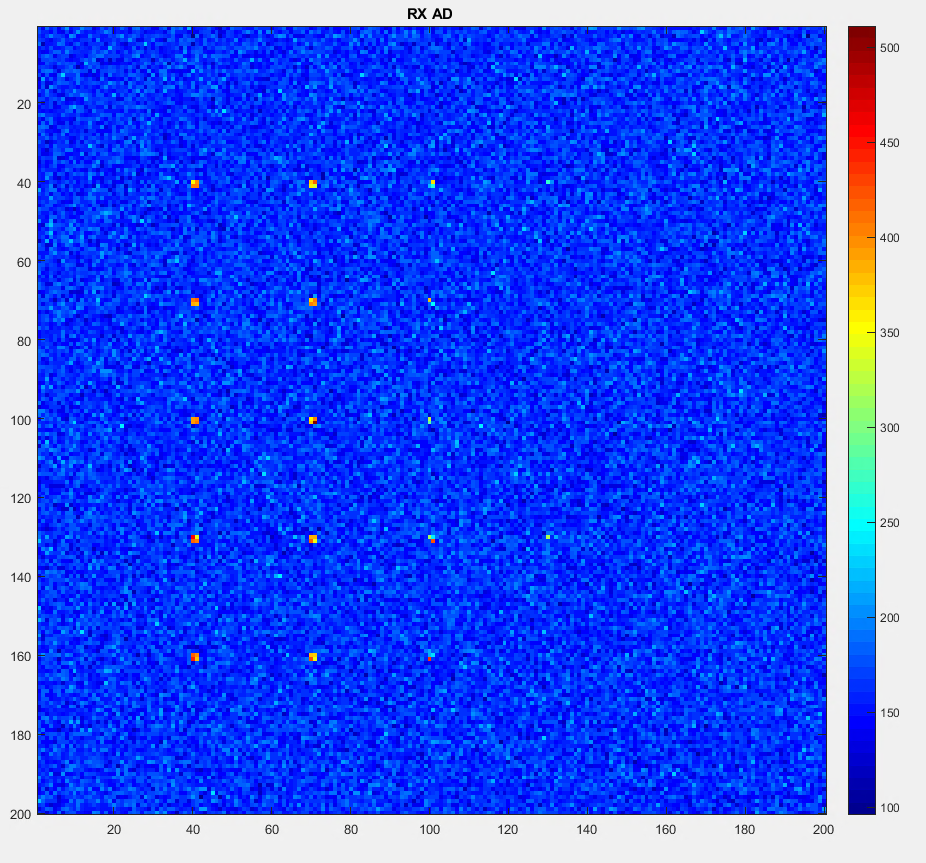
\includegraphics[scale=.35]{images/AD_testing/synthetic_images/rx_ad_hshueh.PNG}}
  %\caption{Lena 256 x 256 uncompressed. Used for testing of MATLAB SPIHT script.}
  %\label{fig:lena_unc}
\end{minipage}%
\begin{minipage}[]{.5\linewidth}
\centering
  \subfloat[Generated anomaly map for RX, setting threshold value for what is considered an anomaly as $\geqslant$ 75\% of the max value of the RX AD.]{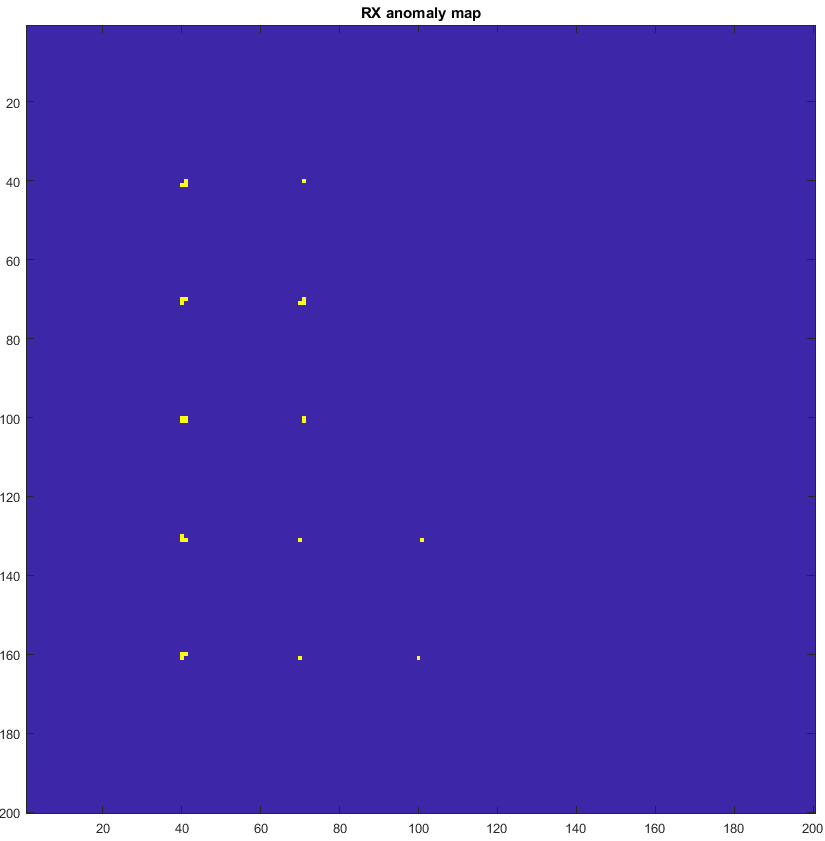
\includegraphics[scale=.3]{images/AD_testing/synthetic_images/rx_hsueh_anomaly_map.PNG}}
  %\caption{Lena 256 x 256 reconstructed after being compressed having 0.1 bpp, using the MATLAB SPIHT script. See appendix. }
  %\label{fig:lena_comp}
\end{minipage}


\caption{RX AD test on synthetic image based on Hsueh's description. The map in (b) was created to provide a way of computing $false\_anomalies$ and $ correctly\_predicted\_anomalies$.  }
\label{fig:hsueh_image_RX_test}
\end{figure}

The value of $false\_anomalies$ = 0, and  $correctly\_predicted\_anomalies$ = $0.3714$ for this test.

\subsubsection{$Sim30\_30AVIRIS$ scene }
\begin{figure}[H]
\centering
   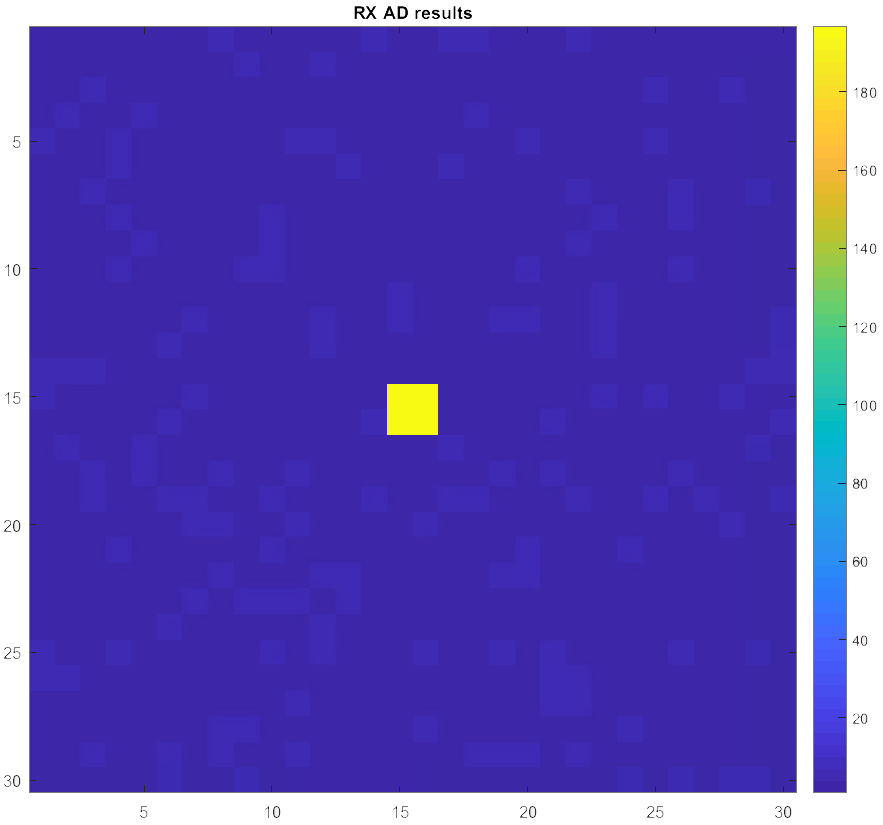
\includegraphics[scale=0.4]{images/AD_testing/synthetic_images/rx_ad_30_30.png}
  \caption{ RX AD results for the $Sim30\_30AVIRIS$ scene.} 
  \label{fig:rx_sim_aviris_30_30}
\end{figure}

The value of $false\_anomalies$ = 0, and  $\%correctly\_predicted\_anomalies$ = $1$ for this test.


\subsubsection{$Sim\_Aviris01$ scene }
\begin{figure}[H]
\hbox{\hspace*{-1cm}                                              
   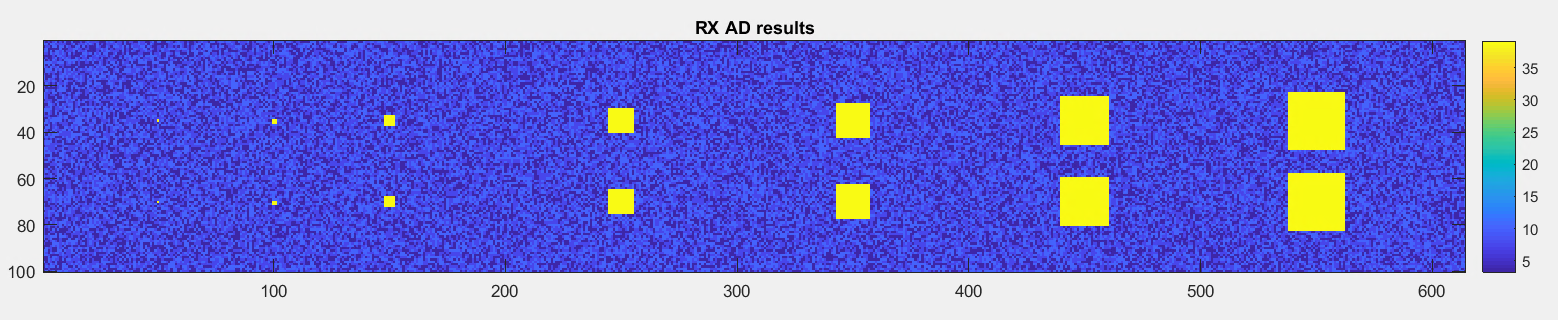
\includegraphics[scale=0.4]{images/AD_testing/synthetic_images/rx_ad_614_100.png}}
  \caption{ RX AD results for the $Sim\_Aviris01$ scene.} 
  \label{fig:rx_sim_aviris_01}
\end{figure}

The value of $false\_anomalies$ = 0, and  $correctly\_predicted\_anomalies$ = $1$ for this test.

\subsection{LRX detection results}
LRX was tested for kernel size $K$=[5, 10, 15, 20, 23, 25 and 30]. These values were chosen as  \cite{global_and_local_rx} tested LRX and optimized the value $K$ empirically, in the range of $K$ =[3,30]. 

\subsubsection{Hsueh mimicked image}

 \begin{table}[H]
\centering
 \resizebox{0.9\textwidth}{!}
{\begin{tabular}{l|l|l}
\textbf{$K$} & $false\_anomalies$ & $correctly\_predicted\_anomalies$\\
5 & 967 &0.0429 \\
10 & 62&0.1143 \\
15 & 58&0.1714 \\
20 & 50& 0.2857\\
23 &46 &0.4782 \\
25 &34 & 0.5143\\
30 & 38& 0.4571\\

\end{tabular}}
\caption{LRX results on Hsueh scene.}
\label{tab:LRX_Hsueh}
\end{table}



\subsubsection{$Sim30\_30 AVIRIS$ scene}
 \begin{table}[H]
\centering
 \resizebox{0.9\textwidth}{!}
{\begin{tabular}{l|l|l}
\textbf{$K$} & $false\_anomalies$ & $correctly\_predicted\_anomalies$\\
5 &12 &0.33 \\
10 &0 &1 \\
15 & 0&1 \\
20 & 0&1 \\
23 &0 &1 \\
25 &0 &1 \\
30 & 0&1 \\

\end{tabular}}
\caption{LRX detection results on $SIM30\_30AVIRIS$ scene.}
\label{tab:LRX}

\end{table}

\subsubsection{$SimAviris01$}
 \begin{table}[H]
\centering
 \resizebox{0.9\textwidth}{!}
{\begin{tabular}{l|l|l}
\textbf{$K$} & $false\_anomalies$ & $correctly\_predicted\_anomalies$\\
5 & 703&0.3562 \\
10 &2584 &0.5106 \\
15 & 2247&0.5621 \\
20 & 2167&0.5710 \\
23 & 1379&0.6737 \\
25 & 1126&0.7192 \\
30 &1056 &0.7208 \\

\end{tabular}}
\caption{LRX results on $SimAviris01$ scene.}
\label{tab:LRX_sim_avirirs01}
\end{table}


\subsection{ALRX detection results}
%\subsubsection{Hsueh mimicked image}
%ALRX was tested for $\tau$ in range [3,100]. 
The threshold $\tau$ in the ALRX algorithm was tested in range [0.5, 100]. The value for $\tau$ yielding best results for $K$ is used in Table \ref{tab:ALRX_simAviris30_30} and \ref{tab:ALRX_simAviris01}. 


\subsubsection{$SIM30\_30AVIRIS$}

 \begin{table}[H]
\centering
 \resizebox{0.9\textwidth}{!}
{\begin{tabular}{l|l|l|l}
\textbf{$\tau$} &\textbf{$K$} & $false\_anomalies$ & $correctly\_predicted\_anomalies$\\
3.5&5 &50 & 0 \\
3.5&10 &46 &0 \\
90&15 & 0&0.5 \\
90&20 & 0&0.5 \\
90&23&0&0.5\\
90&25 &0 &0.5\\
90&30 & 0&0.5 \\

\end{tabular}}
\caption{ALRX results on $SIM30\_30AVIRIS$ scene.}
\label{tab:ALRX_simAviris30_30}
\end{table}



\subsubsection{$SimAviris01$}

 \begin{table}[H]
\centering
 \resizebox{0.9\textwidth}{!}
{\begin{tabular}{l|l|l|l}
\textbf{$\tau$} &\textbf{$K$} & $false\_anomalies$ & $correctly\_predicted\_anomalies$\\
3.5&5 &4760 & 0.3447 \\
3.5&10 &2953 &0.1553 \\
3.5&15 &2871 &0.1252 \\
3.5&20 & 2985&0.0888 \\
%90&23&0&0.5\\
%90&25 &0 &0.5\\
%90&30 & 0&0.5 \\

\end{tabular}}
\caption{ALRX results on $SimAviris01$ scene.}
\label{tab:ALRX_simAviris01}
\end{table}


\subsection{ACAD}
\subsubsection{$SIM\_AVIRIS\_30\_30$}
 \begin{table}[H]
\centering
 \resizebox{0.9\textwidth}{!}
{\begin{tabular}{l|l|l}
\textbf{$\tau$}  & $false\_anomalies$ & $correctly\_predicted\_anomalies$\\
0.1& 8& 0.33 \\
0.3 &6 &0.4 \\
0.5& 4&0.5 \\
0.7& 2&0.6667 \\
0.8&1&0.25\\
0.9 &0 &0\\
1 & 0&0 \\

\end{tabular}}
\caption{ACAD results on $SIM\_AVIRIS\_30\_30$ scene.}
\label{tab:ACAD_simAviris30_30}
\end{table}

%\subsubsection{$SimAviris01$}
% \begin{table}[H]
%\centering
% \resizebox{1.1\textwidth}{!}
%{\begin{tabular}{l|l|l|l}
%\textbf{$\tau$} &\textbf{$k$} & $false\_anomalies$ & $correctly\_predicted\_anomalies$\\
%3.5&5 &50 & 0 \\
%3.5&10 &46 &0 \\
%90&15 & 0&0.5 \\
%90&20 & 0&0.5 \\
%90&23&0&0.5\\
%910&25 & &0.5\\
%3.5&30 & 0&0.5 \\
%
%\end{tabular}}
%\caption{ACAD results on $SimAviris01$ scene.}
%\label{tab:ACAD_simAviris01}
%\end{table}


\section{Testing on real image data}
To evaluate the performance of the ADs considered in this thesis they were tested on hyperspectral image data from the Cuprite mining area captured by the AVIRIS hyperspectral camera.
 Band 220 from Cuprite scene 02 can be seen in figure \ref{fig:cuprite_scene_band_220}.  As no reference anomaly map for this data has been found, it is not possible to calculate $false\_anomalies$ and $correctly\_predicted\_anomalies$. The real image data provides a subjective method of evaluating the performance of the ADs.
% The real image data does not provide means for calculating objective metrics such as $false\_anomalies$ and $\%correctly\_predicted\_anomalies$, but gives an impression of the considered ADs performance when applied to real image data.

\begin{figure}[H]

\hbox{\hspace*{-1.5cm}                                                           

   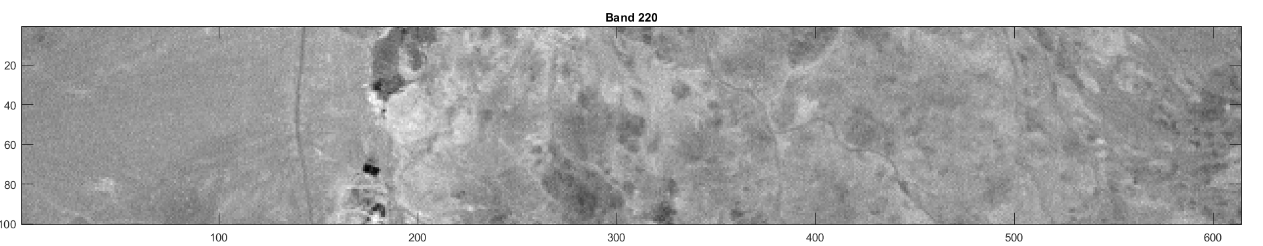
\includegraphics[scale=0.55]{images/AD_testing/original_band_220_22_1.png}}
  \caption{Band 220 from the Cuprite scene 02\cite{Cuprite_data}. } 
  \label{fig:cuprite_scene_band_220}
\end{figure}


\subsection{RX}

Figure \ref{fig:cuprite_scene_rx_result} shows the result of the RX AD on the Cuprite scene 02. A higher score indicates a higher likelihood for the pixel being anomalous.
%As described in section \ref{sec:RX_theory}, the RX algorithm computes the covariance on the global set of pixel vectors to indicate the probability of a pixel being an anomalous pixel. 

\begin{figure}[H]

\hbox{\hspace*{-1cm}                                                           

   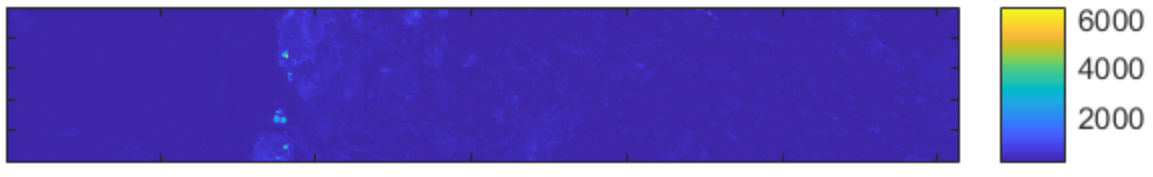
\includegraphics[scale=0.60]{images/AD_testing/rx_detector_result_real_image.PNG}}
  \caption{Result from RX AD on Cuprite image data.  } 
  \label{fig:cuprite_scene_rx_result}
\end{figure}



\subsection{LRX}
Figure \ref{fig:cuprite_scene_lrx_result} shows the result of the LRX AD on the Cuprite scene 02. $K$ = 23 was chosen due to results presented in table \ref{tab:LRX_sim_avirirs01} and the evaluation done in  \cite{global_and_local_rx} which concluded that $K$=23 yielded the best compromise between detection accuracy and computational burden.  
%and results from \cite{chang2006characterization}, which concluded that $k$=25 yielded the best results.

%LRX computes the correlation matrix on a pixel vector block of size $K$ in order to detect anomalous pixel vectors, as described in section \ref{sec:LRX_theory}. 

\begin{figure}[H]

\hbox{\hspace*{-1cm}                                                           

   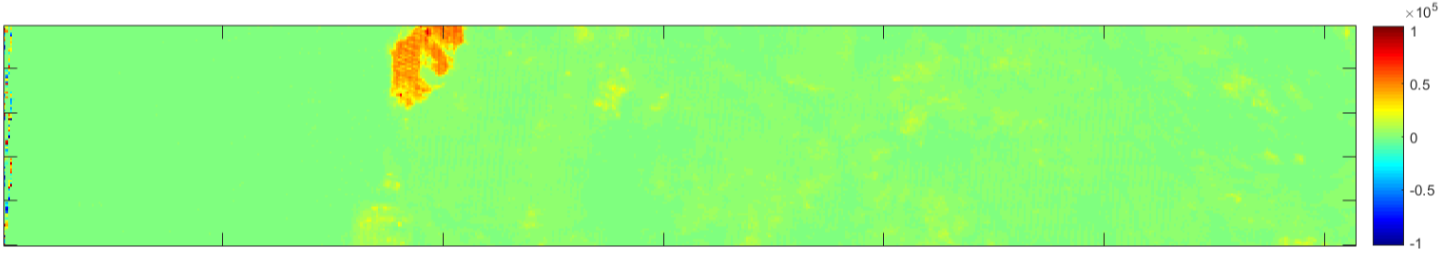
\includegraphics[scale=0.5]{images/AD_testing/hyperspectral_images/real_images/K=23_using_gauss_jordan_colormap_jet.png}}
  \caption{Result from LRX AD with a kernel size of $k$=23 on Cuprite image scene 02. }%Higher score indicates higher probability of the pixel being anomalous. } 
  \label{fig:cuprite_scene_lrx_result}
\end{figure}

%\subsection{ALRX}
%Figure shows the result of the ALRX AD on the Cuprite scene 02. k=23 was chosen results presented in table \ref{tab:LRX_sim_avirirs01} and the evaluation done in  \cite{global_and_local_rx} which concluded that $k$=23 yielded the best compromise between detection accuracy and computational burden. $\tau$ was chosen after expiremental testing. 




\subsection{ACAD}

The resulting anomaly map from ACAD AD on the Cuprite scene 02 is shown in Figure \ref{fig:cuprite_scene_acad_result}. $\tau$ is set to 250. 
%ACAD is causal and computes the correlation matrix on a casual data set, back to the $N_{acad}$ previous pixel. This is further described in section \ref{sec:ACAD_theory}.

\begin{figure}[H]
\hbox{\hspace*{-1.5cm}                                                           

   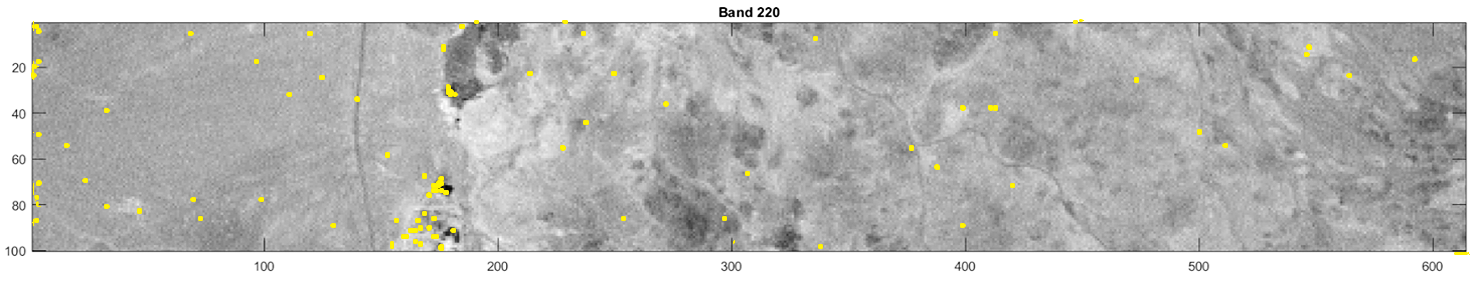
\includegraphics[scale=0.3]{images/AD_testing/anomaly_map_over_picture_tresh=250.png}}
  \caption{Anomaly map created by ACAD( yellow dots) overlayed over Figure \ref{fig:cuprite_scene_band_220}. } 
  \label{fig:cuprite_scene_acad_result}
\end{figure}
 
 \subsection{Choice of anomaly detector algorithm}
 
 Table \ref{tab:ad_comparison} summarizes the comparison of the ADs. 
  
 \begin{table}[H]
\centering
 \resizebox{1.1\textwidth}{!}
{\begin{tabular}{l|l|l|l|l|l}
\textbf{AD}    & \textbf{$false\_anomalies$} &\textbf{ $correctly\_predicted\_$} &\textbf{Performance} & \textbf{Possibility of}  & \textbf{Degree of}                          \\
&(best performance) & \textbf{$anomalies$}& \textbf{on real data}& \textbf{implementing} &\textbf{parallelism}\\
& &(best performance) &  & \textbf{in real time} &\\
\hline
RX & Hsueh : 0&Hsueh: 0.3714 & Figure \ref{fig:cuprite_scene_rx_result}&Low. Need global&Low.Need global\\
&$SIM30\_30AVIRIS:0$ & $Sim30\_30AVIRIS$ : 1 &  & covariance matrix&covariance matrix\\
&$Sim\_Aviris01:0$ & $Sim\_Aviris01$ : 1 & & before computing&before computing \\
& & &  & inverse. &inverse.\\
LRX &Hsueh: 50 & Hsueh: 0.5143 &Figure \ref{fig:cuprite_scene_lrx_result} &Medium. Need to & \\
&$SIM30\_30\_AVIRIS:0 $ & $SIM30\_30\_AVIRIS:1 $ & &wait for a &\\
&$SimAviris01:1056 $ & $SimAviris01:0.7208 $ & & window of size $k$ $\times$ $k$ &\\
& & & &before processing can start & \\ 

ALRX &$SIM30\_30\_AVIRIS:0 $ & $SIM30\_30\_AVIRIS:0.5 $&   &Medium & \\
& $SimAviris01: $ & $SimAviris01: $& &\\
ACAD &Hsueh: &Hsueh: &Figure \ref{fig:cuprite_scene_acad_result} & High. & May pipeline \\
&$SIM30\_30\_AVIRIS:2 $ &$SIM30\_30\_AVIRIS:0.667 $ & & & processing of\\
&$SimAviris01: $&$SimAviris01: $ & & & different pixels.\\
& & & & & 
\end{tabular}}
\caption{Summary of comparison of anomaly detectors.}
\label{tab:ad_comparison}

\end{table}
 
 
 Other metrics are also important to consider in order to choose the best AD for implementation in HW. The ACAD and the ALRX algorithms is beneficial with regards to data transmission requirements, as they build a binary anomaly map of size $N_{pixels}$ $\times$ $N_{rows}$ which may be transmitted, as opposed to RX and LRX algorithms which produces output results of size  $Pixel\_data\_width$ $\times$ 2 $\times$ $N_{pixels}$ $\times$ $N_{rows}$. \\
 
 The ACAD algorithm's causality and the use of correlation matrix makes it easier to process in real time than the LRX and GRX algorithms. ACAD can immediately start processing as the first pixel is captured, while RX, utilizing the global covariance or correlation matrix, cannot start processing until the entire image is captured by the hyperspectral imager. LRX needs an image tile of size $k$ $\times$ $k$ before starting.\\
 
 \cite{chang2006characterization} concludes that ACAD has advantages over the RX AD in several areas. It can be processed in real time. "It detects various anomalies regardless of whether they are of the same type or distinct types" \cite{chang2006characterization}. The above comparison leads to ACAD being chosen as the choice of AD for implementation. 
 
 
 %as the transmitting of a binary anomaly map will require far less than the transmittion of a $n$-bit anomaly detection result.
